% mnras_template.tex 
%
% LaTeX template for creating an MNRAS paper
%
% v3.0 released 14 May 2015
% (version numbers match those of mnras.cls)
%
% Copyright (C) Royal Astronomical Society 2015
% Authors:
% Keith T. Smith (Royal Astronomical Society)

% Change log
%
% v3.0 May 2015
%    Renamed to match the new package name
%    Version number matches mnras.cls
%    A few minor tweaks to wording
% v1.0 September 2013
%    Beta testing only - never publicly released
%    First version: a simple (ish) template for creating an MNRAS paper

%%%%%%%%%%%%%%%%%%%%%%%%%%%%%%%%%%%%%%%%%%%%%%%%%%
% Basic setup. Most papers should leave these options alone.
\documentclass[fleqn,usenatbib]{mnras}

% MNRAS is set in Times font. If you don't have this installed (most LaTeX
% installations will be fine) or prefer the old Computer Modern fonts, comment
% out the following line
\usepackage{newtxtext,newtxmath}
% Depending on your LaTeX fonts installation, you might get better results with one of these:
%\usepackage{mathptmx}
%\usepackage{txfonts}

% Use vector fonts, so it zooms properly in on-screen viewing software
% Don't change these lines unless you know what you are doing
\usepackage[T1]{fontenc}

% Allow "Thomas van Noord" and "Simon de Laguarde" and alike to be sorted by "N" and "L" etc. in the bibliography.
% Write the name in the bibliography as "\VAN{Noord}{Van}{van} Noord, Thomas"
\DeclareRobustCommand{\VAN}[3]{#2}
\let\VANthebibliography\thebibliography
\def\thebibliography{\DeclareRobustCommand{\VAN}[3]{##3}\VANthebibliography}


%%%%% AUTHORS - PLACE YOUR OWN PACKAGES HERE %%%%%

% Only include extra packages if you really need them. Common packages are:
\usepackage{graphicx}	% Including figure files
\usepackage{amsmath}	% Advanced maths commands
\usepackage{amssymb}	% Extra maths symbols

%%%%%%%%%%%%%%%%%%%%%%%%%%%%%%%%%%%%%%%%%%%%%%%%%%

%%%%% AUTHORS - PLACE YOUR OWN COMMANDS HERE %%%%%

% Please keep new commands to a minimum, and use \newcommand not \def to avoid
% overwriting existing commands. Example:
%\newcommand{\pcm}{\,cm$^{-2}$}	% per cm-squared

%%%%%%%%%%%%%%%%%%%%%%%%%%%%%%%%%%%%%%%%%%%%%%%%%%

%%%%%%%%%%%%%%%%%%% TITLE PAGE %%%%%%%%%%%%%%%%%%%

% Title of the paper, and the short title which is used in the headers.
% Keep the title short and informative.
\title[Rates of SNe Ia in DES]{Rates and delay times of type Ia supernovae in the Dark Energy Survey}

% The list of authors, and the short list which is used in the headers.
% If you need two or more lines of authors, add an extra line using \newauthor
\author[P. Wiseman et al.]{
P. Wiseman,$^{1}$\thanks{E-mail: p.s.wiseman@soton.ac.uk}
A. N. Other,$^{2}$
Third Author$^{2,3}$
and Fourth Author$^{3}$
\\
}

% These dates will be filled out by the publisher
\date{Accepted XXX. Received YYY; in original form ZZZ}

% Enter the current year, for the copyright statements etc.
\pubyear{2020}

% Don't change these lines
\begin{document}
\label{firstpage}
\pagerange{\pageref{firstpage}--\pageref{lastpage}}
\maketitle

% Abstract of the paper
\begin{abstract}
We use a sample of 881 photometrically classified SNe discovered by the Dark Energy Survey (DES) in the redshift range $0.2 < z <0.6$, along with 40415 field galaxies to calculate the rate of type Ia supernovae (SNe Ia) per galaxy. We recover the established positive trend of SN Ia rate as a function of galaxy stellar mass across a broad range of scales $8.5 \leq \log(M_*/\mathrm{M}_{\odot}) \leq 11.25$. We find that the SN Ia rate increases with stellar mass roughly linearly in log space, with a slope of $0.63 \pm 0.02$, which is consistent with previous work. We use an empirical model of stellar mass assembly to estimate the average star-formation histories (SFHs) of galaxies across the stellar mass range of our measurement. Combining the modelled SFHs with the SN Ia rates to estimate constraints on the SN Ia delay time distribution (DTD), we find the data are best fit by a power-law DTD with index $\beta = -1.14 \pm 0.05$ and normalisation $A = 2.1 \pm0.05 \times 10^{-13}~\mathrm{SNe}~{\mathrm{M}_{\odot}}^{-1}~\mathrm{yr}^{-1}$. Upon splitting the SN sample by properties of the light curves, we find a strong dependence on DTD slope with the SN stretch parameter, with slower-declining SNe exhibiting a steeper DTD slope.
\end{abstract}

% Select between one and six entries from the list of approved keywords.
% Don't make up new ones.
\begin{keywords}
keyword1 -- keyword2 -- keyword3
\end{keywords}

%%%%%%%%%%%%%%%%%%%%%%%%%%%%%%%%%%%%%%%%%%%%%%%%%%

%%%%%%%%%%%%%%%%% BODY OF PAPER %%%%%%%%%%%%%%%%%%

\section{Introduction}

Type Ia supernovae (SNe Ia) are explosions of white dwarves (WDs) at masses close to the Chandrasekhar limit of 1.44 $M_{\odot}$. The small observed dispersion in their peak brightnesses can be reduced further through empirical relations between brightness and light curve properties, such as decline rate (stretch) or optical colour. These properties have led SNe Ia to be used extensively by cosmologists to measure relative distances in the Universe.

Despite reducing dispersions to $\sim 0.1$ mag in samples with over one thousand SNe \citep{Scolnic2018}, the exact nature of the progenitor scenarios for SNe Ia is yet to be confirmed. While it is accepted that SNe Ia are caused by accretion of matter onto a WD from a companion star, multiple possible scenarios exist for the nature of that companion star and the search for this has formed a significant field of research (see \citealt{Maoz2014} for a review). The leading models involve a main sequence (MS) star in the single-degenerate (SD) scenario \citep{Whelan1973,Nomoto1982}, a secondary white dwarf in the double-degenerate (DD) scenario \citep{Tutukov1976,Iben1984,Webbink1984}, while more exotic models such as the core-degenerate (CD) scenario invoke white dwarves merging with the cores of massive stars \citep{Soker2019}. 

The progenitors of a number of core-collapse SNe (CCSNe) have been identified in high-resolution pre-explosion images, allowing detailed analysis of the latter stages of massive star evolution. However, this approach has not yet been successful in identifying a progenitor of a SN Ia. Conversely, it has been possible to search for surviving remnants of the binary system -- main sequence stars or white dwarves left behind at the SN location or kicked \citep{Shen2018} -- displaying tentative evidence for a DD scenario. As yet, there is no conclusive evidence ruling out any progenitor channel from being a significant contribution to the total population of SNe Ia.

Another method of inferring progenitor channels is the study of the SN Ia delay time distribution (DTD). The DTD can be interpreted as the rate at which SNe Ia occur as a function of the delay time $\tau$ since an episode of star-formation, and thus carries characteristic signatures of the progenitor channel (see \citealt{Wang2012} for a review). While the SD scenario is able to produce a broad range of functional forms of the DTD, the DD scenario predicts a power law of the form $\tau^{\beta}$, with $\beta \sim -1$ \citep[e.g][]{Ruiter2009,Mennekens2010}.

A power law DTD implies that most SNe Ia explode soon after star formation, but also that there is a non-neglible fraction that explode on the order of Gyrs after the star formation episode. The DTD is therefore non-trivial to measure and various techniques have been developed to infer it indirectly. One such approach is to measure global properties of SN Ia host galaxies. Simple examples of such analyses are comparisons of the rates of SNe Ia in hosts that have been split by some observational property, such as morphology or colour, and have shown that SNe Ia rate per unit stellar mass (SNuM) is significantly larger in late-type spiral galaxies as well as in bluer galaxies \citep[e.g.][]{Mannucci2005}. These observations heavily imply that SNe Ia rates are dependent on recent or ongoing star-formation, and thus that the majority of SNe Ia explode after short delay times. Conversely, the SNuM in E/S0 and red galaxies is non-negligible, suggesting that there is a secondary, much older component to the DTD \citep{Sullivan2006,Smith2012}. The DTD is thus approximated by a two-component ("$A + B$") model, where $A$ and $B$ are the normalizations of the DTD for "prompt" (i.e. proportional to instantaneous SFR) and "tardy" (i.e. proportional to overall stellar mass) SNe, respectively.

A complementary technique involves measuring the evolution of the volumetric rate of SNe Ia as a function of redshift and comparing this evolution to the average cosmic star-formation history (CSFH) of the Universe \citep{Gal-Yam2004,Strolger2004,Dahlen2004,Dahlen2008, Graur2013, Frohmaier2019}. This technique (the volumetric rate method) is also applicable to galaxy clusters, for which it is assumed that the star-formation histories are strongly peaked at some past epoch and thus that the rate of SNe Ia in clusters as a function of redshift is a more direct measure of the DTD \citep{Maoz2004,Graur2014,Maoz2014}. These studies have, almost ubiquitously, found $\beta$ to be consistent with $-1$.

It is also possible to estimate the SFH of an individual galaxy through the modelling of its stellar populations via spectral energy distribution (SED) fitting. Works such as \citet{Maoz2011}, \citet{Maoz2012} and \citet{Graur2013} estimated the DTD by measuring SFHs for a sample of field galaxies and comparing them to the number of SNe detected in each galaxy (the SFHR method), and have led to results that suggest a DTD power law with $\beta$ consistent with $-1$ \citep[e.g.][]{Maoz2011,Graur2013}. \citet{Childress2014} showed that the $A+B$ parameterisation arises as a direct consequence of the combination of a power-law DTD with the SFHs of galaxies. The recent advances of integral field spectroscopy (IFS) allows for an extension of the SFHR method, by reconstructing the SFH for hundreds or thousands of local regions of each SN Ia host galaxy. Using this method, \citet{Castrillo2020} find a power-law slope of $-1.1\pm0.3$, while \citet{Chen2021} find $-1.4\pm0.3$.

In this work, we combine parts of the above methods and derive a new, independent measurement of the SN Ia DTD. Instead of measuring the volumetric rate of SNe Ia, we measure the rate per galaxy as a function of stellar mass, as per \citet{Sullivan2006,Smith2012}. We use the stellar mass assembly model of \citet{Childress2014} to predict the stellar age distribution of galaxies for a given stellar mass at the mean redshift of our SN sample, and then forward model the DTD by convolving it with the stellar age distribution and comparing the predicted rates to the observed rates.

We introduce the SN host and field galaxy samples in Section \ref{sec:data} and describe our handling of incompleteness in Section \ref{sec:incompleteness}. We present the SN Ia rate per galaxy in Section \ref{sec:rates}. We outline the modelling of star-formation histories and measurement of the DTD in Section \ref{sec:model} before concluding in Section \ref{sec:conclusion}.
Where relevant, we assume a spatially flat $\Lambda$CDM cosmology with $\Omega_m = 0.3$ and $H_0 = 70 \mathrm{ km s}^{-1}\mathrm{Mpc}^{-1}$. Unless otherwise stated, we assume Gaussian uncertainties quoted at the $1\sigma$ level. Magnitudes are quoted in the AB system \citep{Oke1983}.


\begin{table}
	\centering
	\caption{Numbers of field galaxies and SN hosts passing various quality cuts.}
	\label{tab:cuts}
	\begin{tabular}{lccr} % four columns, alignment for each
		\hline
		Cut & N (field galaxies)  & N (SN hosts)\\
		\hline
		Chosen fields & 1364311  & 1766\\
	    Kron mag in all bands & 1069004  & 1764 \\
	    Masked chips & 816950  & - \\
	    Has ugrizJHK photometry & 545748  & -\\
	    Edge of chip & 481731 & 1716 \\
	    Star/galaxy separation & 400051 &  1678\\
	    Has good redshift & 395034 & 1678 \\
	    SNR $\geq 3$& 338256  & 1678 \\
	    $m_r \leq 24.5$ & 196109 &  1678 \\
	    $0.2 \leq z \leq 0.8$ & 48177 & 1414\\ 
	    
		\hline
	\end{tabular}
\end{table}

%%%% DATA %%%%
\section{Data}

In order to measure the rate of SNe Ia per galaxy per year, we require a sample of SNe Ia and a sample of field galaxies that are normalised to the same selection criteria -- the final rate calculation must be corrected for differences in sky area, redshift depth, and survey time. In this section, we introduce our SN and field galaxy samples.


\label{sec:data}
\subsection{Dark Energy Survey supernova programme \label{subsec:des}}
The DES Supernova Programme (DES-SN) is a transient survey based on five six-month seasons of observations with the Dark Energy Camera (DECam; \citealt{Flaugher2015}), designed primarily to measure the light curves of SNe Ia for use as cosmological distance indicators. Transients were detected and processed using a difference imaging program \citep{Kessler2015} and vetted using a machine learning (ML) algorithm \citep{Goldstein2015}. Spectral follow-up was performed on a suite of large optical telescopes \citet{Smith2020a}, leading to the initial publication of a measurement of cosmological parameters using 207 spectroscopically confirmed SNe (\citealt{DESCollaboration2018a}, and references therein). 
\subsection{Supernovae \label{subsec:host_sample}}
\subsubsection{Photometric classification and quality cuts \label{subsubsec:sn_classify}}
With over 30,000 transients passing ML cuts it was not possible to obtain spectral follow up of every object. Instead we make use of photometric classification techniques, in particular the recurrent neural network classifier \texttt{superNNova} (SNN; \citealt{Moller2019}). We derive our SN Ia sample following the approach of \citet{Scolnic2020}, but use a threshold probability of $P(\mathrm{Ia})\geq0.5)$. The photometricially classified SNe Ia are then passed through the \texttt{SALT2} framework \citep{Betoule2014} and are subject to quality cuts on the light curve width (stretch; $x_1$) and colour ($c$) parameters in an identical manner to \citet{Vincenzi2020}: $-3 \leq x_1 \leq 3$, $-0.3 \leq c \leq 0.3$. These cuts help to reduce the potential contamination from core-collapse SNe (CCSNe) and outlying thermonuclear SNe. We impose further cuts on the quality of those measured parameters, which are: the uncertainty on $x_1$: $\sigma_{x_1} <1$; the uncertainty on the date at which the light curve peaked: $\sigma_{t_{\mathrm{peak}}} <2$; the SALT2 fit probability $>0.001$.  % whose physical mechanisms may diverge from the general cosmologically useful population.

\subsubsection{Host galaxy selection \label{subsubsec:sn_hosts}}
Host galaxies for all transients in DES-SN are derived from the deep-stacked $g, r, i, z$-band images presented in \citet{Wiseman2020}. SN are associated to hosts using the directional light radius method \citep[e.g.][]{Sullivan2006,Gupta2016}, while spectroscopic redshifts are provided by OzDES \citep{Yuan2015,Childress2017,Lidman2020}, leading to an initial sample of 1766 SNe.

\subsection{Field galaxies\label{subsec:field_sample}}
Along with a sample of SNe, we also require a sample of field galaxies in order to determine a per-galaxy rate. In order to maintain consistency between the SN host and field galaxy sample selections, we obtain a field galaxy sample from the same catalogue as that from which the SNe are matched to obtain host galaxies. The steps relevant to this analysis are outlined in the following sections.

\subsubsection{Photometric redshifts \label{subsubsec:photozs}}

Since the vast majority of objects detected in the deep photometry do not have a spectroscopic redshift measurement, we rely on photometric redshifts (photo-$z$s) in order to proceed with the analysis. 
Photometric redshifts are taken, where available, from the catalogue of \citet{Hartley2020}, and have been estimated using the \texttt{EAZY} photometric redshift code \citep{Brammer2008}. These photo-$z$s make use of deep DES optical photometry alongside DECam $u$-band data and near-infrared (NIR) $J$, $H$, and $K$-band imaging from the ultraVISTA and VIDEO surveys. Photo-$z$ accuracy from \citet{Hartley2020} at $17 < i<24$, as quantified by the Normalised Absolute Median Deviation (NMAD) is estimated around 0.03. This accuracy is degraded to 0.07 at $17 < i<26$, a range that includes all galaxies in our sample, but is more than adequate for the purposes of this work, where all field galaxies will be grouped into stellar mass bins of 0.5 dex.

\begin{figure}
    \centering
    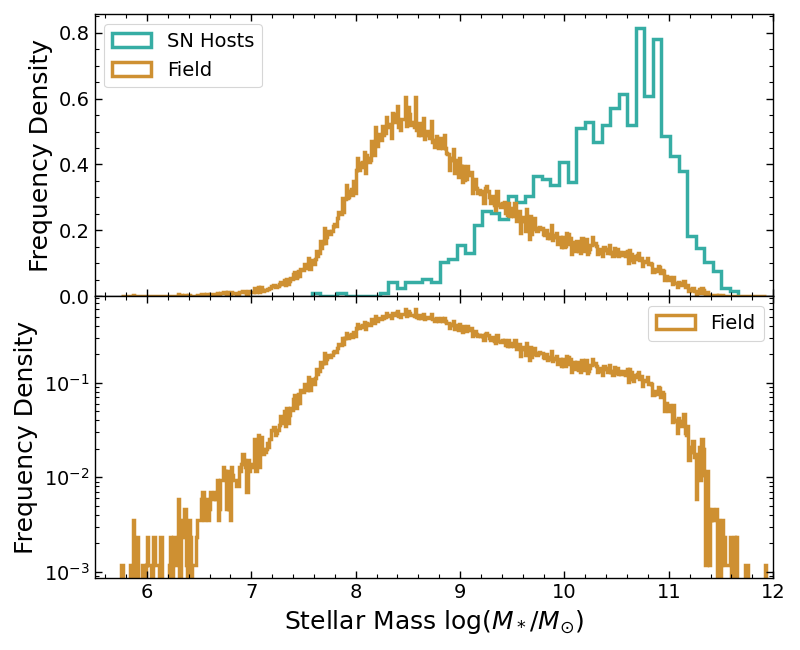
\includegraphics[width=.5\textwidth]{figs/mass_hist_linlog_sn_field_BC03.png}
    \caption{Upper: Distribution of the stellar mass of the SN host (green dot-dashed) and field galaxies (orange solid) used in the analysis. Lower: As upper for field galaxies, but shown on a log scale.  The distribution closely matches data from the ZFOURGE survey at $0.2<z<0.5$ (cyan dashes) and $0.5<z<0.75$ (magenta dots).}
    \label{fig:mass_hist_hosts_field}
\end{figure}


\begin{figure}
    \centering
    %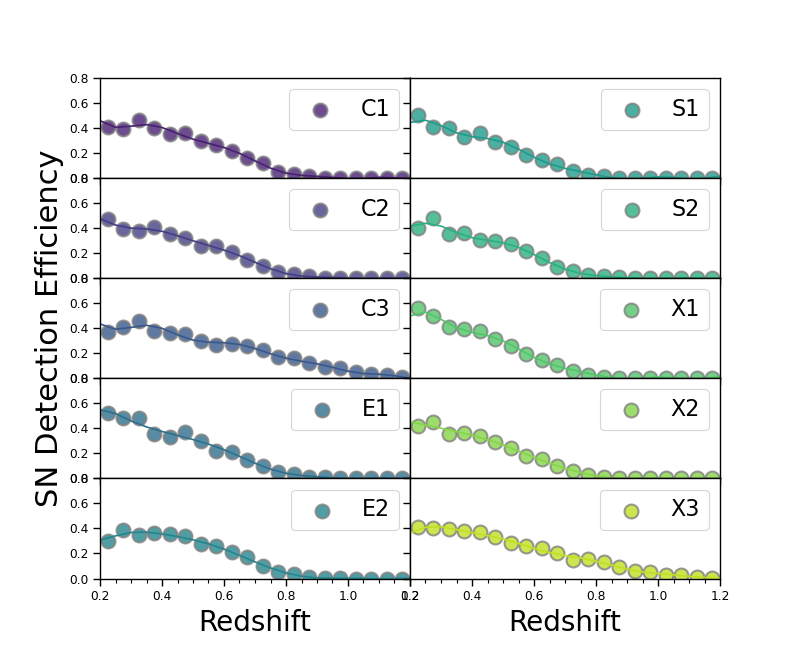
\includegraphics[width=0.5\textwidth]{figs/SN_efficiencies.png}
    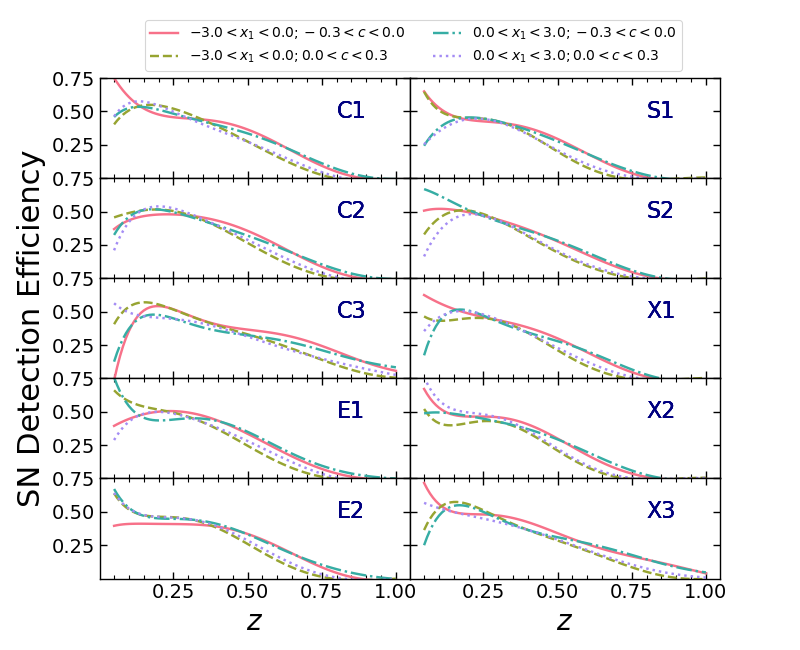
\includegraphics[width=0.5\textwidth]{figs/SN_efficiencies_z_x1_c.png}
    \caption{ SN detection efficiencies split by DES-SN field, $x_1$ and $c$. The $y-$axis represents the fraction of simulated SNe in a given redshift bin that would have been detected by DES-SN and passed light curve quality cuts. Lines are polynomial fits that approximate the efficiency curves. 
    \label{fig:SN_efficiency}}
\end{figure}

\begin{figure}
    \centering
    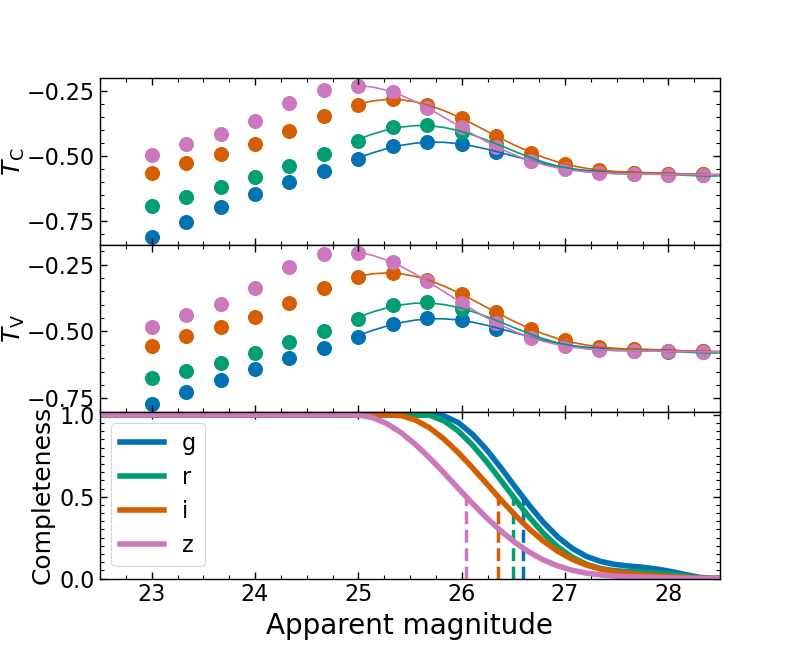
\includegraphics[width=0.5\textwidth]{figs/completeness_combined.png}
    \caption{Measuring the completeness of the field galaxy sample. \textit{Upper}: the $T_{\mathrm{C}}$ statistic as a function of apparent magnitude; \textit{middle} as per \textit{upper}, but for $T_{\mathrm{V}}$; \textit{lower}: the combined, normalised completeness in each band.  
    \label{fig:completeness}}
\end{figure}

\begin{figure}
    \centering
    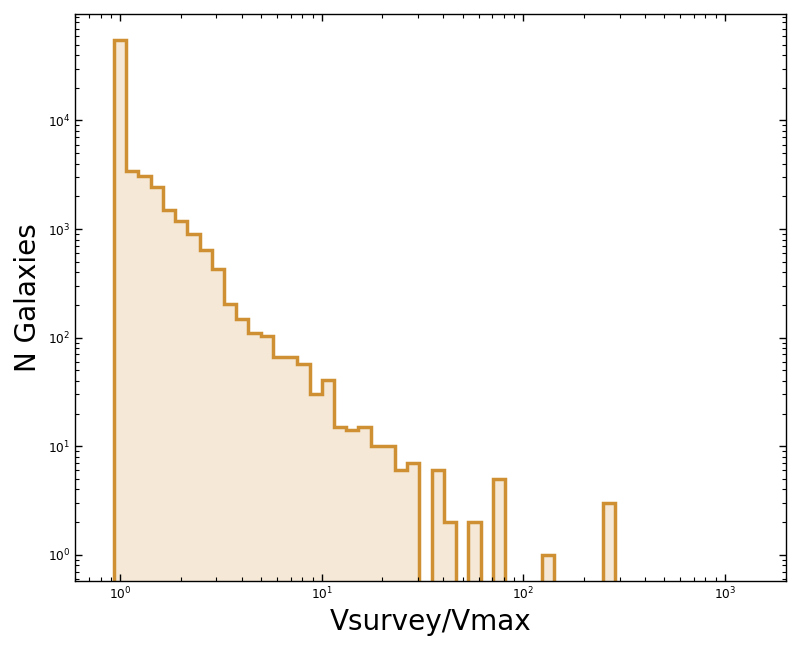
\includegraphics[width=0.5\textwidth]{figs/field_vmax.png}
    \caption{Distribution of $V_{\mathrm{max}}$ corrections applied to field galaxies in the DES sample. The majority of galaxies have no correction, and the distribution of the 1\% that do follows a power-law.
    \label{fig:vmax_field}}
\end{figure}

\subsection{Quality cuts \label{subsec:cuts}}

In order to refine the sample of host and field galaxies for the rate analysis we perform a series of quality cuts:

\begin{enumerate}
    \item[i)] objects must be detected and have a Kron magnitude measurement in all four DES optical bands
    
    \item[ii)] field galaxies are limited to unmasked region of the SN-X3 chip \cite{Hartley2020}
    
    \item[iii)] objects must not be within a given number (20 in $x$, 50 in $y$) of pixels of the CCD edge, as the co-addition of slightly misaligned images introduced a region of significant noise in this part of the detector
    
    \item[iv)] objects must have a value of 0.95 in the star/galaxy (S/G) separation \texttt{CLASS\_STAR} provided by \texttt{Source Extractor} \citep{Bertin1996}
    
    \item[v)]  objects must be covered by $ugrizJHK$ photometry with either detections or upper limits
    
    \item[vi)] objects must have a spectroscopic or photometric redshift measurement
    
    \item[vii)] objects must be detected at signal-to-noise ratio (SNR) greater than 3 in the $r$ band
    
    \item[viii)] galaxies must be brighter than $m_r \leq 24.5$, as this is the magnitude of the faintest SN host with a spectroscopic redshift.
    
    \item[ix)] galaxies must be within the redshift range $0.2 \leq z \leq 0.6$ (see Section \ref{subsec:incompleteness_SNe} for an explanation of this cut).
\end{enumerate}

The numbers of SN hosts and field galaxies passing these cuts are listed in Table \ref{tab:cuts}. The final samples comprise 1204 SN host galaxies and 48,177 field galaxies. The volume-weighted mean redshifts are 0.65 and 0.63 for SNe and field galaxies, respectively.

\subsection{Galaxy properties \label{subsec:properties}}

We estimate global galaxy properties for both the SN host and field galaxies that pass the quality cuts by fitting the photometry with stellar population templates in a method outlined by \citet{Sullivan2006} and consistent to that used in previous DES-SN analyses \citep{Kelsey2020,Smith2020,Wiseman2020}. For SN hosts the redshift is fixed at the spectroscopically determined value, while for field galaxies we fix it at either the spectroscopic value if one exists in the OzDES Global Redshift Catalog \citep{Lidman2020}, or more commonly the photometrically derived value. We use the stellar population templates of \citet{Bruzual2003} and adopt a \citet{Chabrier2003} initial mass function (IMF). The fitting procedure returns a best fitting template and corresponding stellar mass ($M_*$). Upper and lower bounds on stellar mass estimates are taken as the largest and smallest values of a given parameter for which the reduced $\chi^2$ parameter corresponds to $\chi^2_{\mathrm{red, min}} +1$. 

The results of our SED fitting are shown in Fig. \ref{fig:mass_hist_hosts_field}. The upper panel, with both the SN hosts and field galaxies displayed, shows the vastly different distributions of the two samples. SN hosts are preferentially high mass galaxies, whereas the field galaxy distributions increases down to lower masses, peaking around $10^{8.5}~\mathrm{M}_{\odot}$. In the bottom panel, the same field galaxy stellar mass distribution is shown on a log scale, along with the stellar mass function (SMF) from the ZFOURGE survey \citep{Tomczak2014} that best represents the redshift range of the DES field galaxies. Above $10^{8.5}~\mathrm{M}_{\odot}$, the DES field galaxy distribution closely follows the ZFOURGE SMF for $0.5<z<0.75$, indicating that the DES sample is representative of field galaxies in this redshift range.%To estimate uncertainties on the physical properties, we resample the photometry from a Gaussian distribution formed by the flux measurements and their uncertainties and rerun the SED fit. This procedure is repeated 1000 times. 
%%%% INCOMPLETENESS %%%%


\section{Incompleteness corrections}
\label{sec:incompleteness}
The simple ratio of the number of SN hosts and field galaxies presented at the end of the previous section provides a first approximation of the SN rate per galaxy, and the addition of factor equal to the survey duration normalises the rate to per year. However both the SN and field galaxy samples introduced in Sections \ref{subsec:host_sample} and \ref{subsec:field_sample} are affected by incompleteness, which is likely to be the dominant systematic effect in the analysis. In this section we describe our method of correcting for various sources incompleteness in the data.

\subsection{Supernovae \label{subsec:incompleteness_SNe}}

Incompleteness in a SN survey arises from a number of sources. The primary source of incompleteness is caused by the magnitude limit of the survey: SNe with apparent magnitudes below the survey limit will not be detected. Since SNe Ia are relatively uniform in absolute luminosity, this form of incompleteness is primarily redshift dependent. On the other hand, DES-SN comprises 10 separate pointings, each with different visibility and thus airmass throughout the observing season. These differences lead to different detection efficiencies across the fields.

To correct for these incompleteness, we follow a similar method to that used in the PTF rates analyses of \citet{Frohmaier2019,Frohmaier2020} as well as the DES-SN superluminous SN rate of \citet{Thomas2020}. We run a suite of simulations using an identical method to that described in detail in \citet{Vincenzi2020}. We simulate SNe using the SuperNova ANAlysis software (\texttt{SNANA} \citealt{Kessler2009a}) integrated into the \texttt{pippin} framework \citep{Hinton2020}. We simulate 230,000 SNe in the redshift range $0.05 \leq z_{\mathrm{SN}} \leq 1.3$. The SNe are generated with SEDs based upon the SALT2 model \citep{Guy2007} and trained on the Joint Lightcurve Analysis dataset \citep{Betoule2014}. The SALT2 parameters $x_1$ (stretch) and $c$ (colour) are drawn randomly from the intrinsic asymmetric Gaussian distributions described in \citet{Scolnic2016} and "blurred" following the intrinsic scatter model of \citet{Guy2010}, while redshifts are drawn following the volumetric rate evolution of \citet{Frohmaier2019}. The SNe are simulated with explosion epochs $t_0$ uniformly distributed between two months before DES-SN began and two months after it finished. We run mock versions of the DES-SN survey, using the exact cadence, conditions, and zeropoints from the survey itself. All of the detected simulated SNe are passed through the light curve fit of SALT2 \citep{Betoule2014}, as per the implementation in \texttt{SNANA}, and those that fail the light curve cuts outlined in Section \ref{subsubsec:sn_classify} are discarded. We are left with a fraction of the original simulated SNe, and that fraction is dependent on a combination of sky location, explosion epoch, redshift, stretch, and colour. The fraction of recovered SNe (the efficiency) is thus described by a 5-dimensional surface. For the $i$th SN the efficiency $\eta_{\mathrm{SN}, i}$ in field $F$, exploding at time $t_0$ at redshift $z$, with stretch $x_1$ and colour $c$, is:
\begin{equation}
    \eta_{\mathrm{SN},i} (F_i,z_i,t_{0,i},x_1,c) = \left( \frac{N_{\mathrm{obs}}\left(F_i,z_i,t_{0,i},x_1,c\right)}{N_{\mathrm{sim}}\left(F_i,z_i,t_{0,i},x_{1,i},c_i\right)}\right)\,.
\end{equation}

In practice, the gradient of the efficiency function is strongest between different DES fields and as a function of redshift, while SN stretch and colour have smaller effects. We integrate the efficiencies across the full simulated time range, and as such the efficiency is limited to $\sim 0.5$ due to the 6-month nature of the DES observing seasons.
The distribution of efficiency as a function of redshift is shown in Figure \ref{fig:SN_efficiency}. It is evident that the deep fields (X3, C3) are sensitive to SNe at higher redshifts, while there is no drastic shifts between efficiencies in the eight shallow fields. There is evidence that the SN efficiency depends weakly on $x_1$ and more strongly on $c$, which is expected since the colour correction term is larger than the stretch correction term in the SN Ia standardisation formula \citep{Tripp1998}. Blue SNe are recovered more readily than red SNe as they are generally brighter. 

The deep fields show non-zero efficiencies approaching $z=1$, whereas the shallow fields typically reach $z=0.8$. Since fractional uncertainty is large at such low efficiencies, we choose to make a redshift cut of $z=0.6$ where the efficiency is well above 0.1 in all fields. 

\subsection{Supernova hosts \label{subsec:incompletenss_SN_hosts}}
A further limiting factor in the SN host sample is the requirement of a spectroscopic redshift. The majority of SN host spectroscopic redshifts in DES are provided by the dedicated follow-up survey OzDES, for which the limiting magnitude is around 24 to 24.5 mag in the $r$ band. The rate at which a host redshift is successfully measured given an apparent magnitude has been extensively modelled by \citet{Vincenzi2020} who provide the spectroscopic redshift efficiency as a function of host $r$-band magnitude, host galaxy colour, and the year in which the SN was discovered in order to allow for a longer possible spectroscopic exposure time for hosts of SNe discovered earlier in the survey. So that we reduce any bias towards SNe in bright hosts that are easier to obtain spectroscopic redshifts for, we assign each SN in the sample described in Section \ref{subsec:host_sample} a weight equal to the inverse of the spectroscopic efficiency for its host. This is equivalent to assuming that an efficiency of 0.1 means that for every ten SNe with hosts at that magnitude, only 1 will make it into the sample.

\subsection{Field galaxies \label{subsec:incompleteness_field}}

\subsubsection{Apparent magnitude limits \label{subsubsec:mag_lims}}
As we use photometric, rather than spectroscopic, redshifts for the field galaxies, they do not suffer from spectroscopic incompleteness as the SN hosts do. Instead, the inclusion of any given galaxy in the survey area in the sample is determined simply by whether it is detected above a prescribed threshold in signal-to-noise ratio, i.e. the sample is magnitude limited. To determine the apparent magnitude limit in each of the optical bands we employ the method of \citet{Johnston2007,Teodoro2010,Johnston2012} (hereafter Completeness I, II, III respectively). Test statistics $T_{\mathrm{C}}$ and $T_{\mathrm{V}}$ are computed based on absolute magnitude and distance modulus by calculating the rank of each galaxy's absolute magnitude (distance modulus) when compared to all other galaxies in a survey within a certain slice of distance modulus (absolute magnitude). For a galaxy of apparent magnitude $m < m_{\mathrm{lim, trial}}$ observed in a survey complete to magnitude $m_{\mathrm{lim, true}}$ where  $m_{\mathrm{lim, trial}} \leq m_{\mathrm{lim, true}}$, the expectation value of the rank is 0.5. However, if a trial limiting magnitude $m_{\mathrm{lim, trial}} \geq m_{\mathrm{lim, true}}$, there will be a lack of observed faint objects, such that the expectation value of the rank drops. Completeness I, II, and III show that for surveys with sharp, well defined magnitude limits the test statistics $T_{\mathrm{C}}$ and $T_{\mathrm{V}}$ drop sharply. The DES deep stacks present a more challenging case. They cover a wide area and are compiled from tens of separate CCDs, each with its own detection efficiency. Moreover, galaxy redshifts have been estimated using photometry only, and $K$-corrections performed using an imperfect template fit, potentially leading to large systematic and statistical fluctuations in absolute magnitudes and distance moduli. To reduce the inhomogeneity while still including  large sample of objects, we split the sample into the deep (X3) and shallow (E2) fields and calculate limiting magnitudes separately. Fig. \ref{fig:completeness} shows the values of $T_{\mathrm{C}}$ and $T_{\mathrm{V}}$. The values of the test statistics increase with $m_{\mathrm{lim, trial}}$ until a peak, before decreasing to stable values at magnitudes far beyond the limit of the survey. The shape at brighter $m_{\mathrm{lim, trial}}$ is likely caused by incompleteness at the bright end: due to the small sky area, we simply do not probe enough volume to sample the bright end of the galaxy luminosity function well enough for the statistics to be robust. To approximate an efficiency function, we fit the peak of the statistics with a polynomial function, and then normalise by the maximum and minimum values. We then interpolate between the peak and the faint-magnitude floor to find the 50\% completeness limit at the point where the normalised value of the test statistic is 0.5. These values are consistent with the value at which 50\% of the true sources are detected but have the advantage of being derived from the data without a simulation that is based on assumptions and thus susceptible to bias.

\subsubsection{$V_{\mathrm{max}}$ correction \label{subsubsec:vmax_corr}}

To correct for incompleteness caused by the magnitude limited nature of the survey we follow the prescription of e.g. \citet{Sullivan2006, Smith2012} by using a $V_{\mathrm{max}}$ method based on \citet{Schmidt1968}. For each galaxy in the sample we calculate the maximum volume within which it would have been observed given its absolute magnitude and $k-$correction. A correction of $V_{\mathrm{survey}}/V_{\mathrm{max}}$ is applied to all galaxies for which $V_{\mathrm{max}} < V_{\mathrm{survey}}$, where $V_{\mathrm{survey}}$ is the maximum volume reached by the survey. In our case this corresponds to the volume at $z=0.8$. Fig \ref{fig:vmax_field} shows the distribution of the correction among galaxies in the sample. The vast majority of galaxies require no correction, meaning they would have been observed beyond the maximum volume considered. Roughly 1\% of objects have a correction greater than 1, with the distribution well described by a power-law function.

%In Section \ref{sec:rates} we split the samples into redshift bins in order to measure cosmic evolution of the SN Ia rate. For each redshift bin, we reevaluate the value of $V_{\mathrm{survey}}$ used in the incompleteness correction to be the volume of the bin.


\begin{figure}
    \centering
    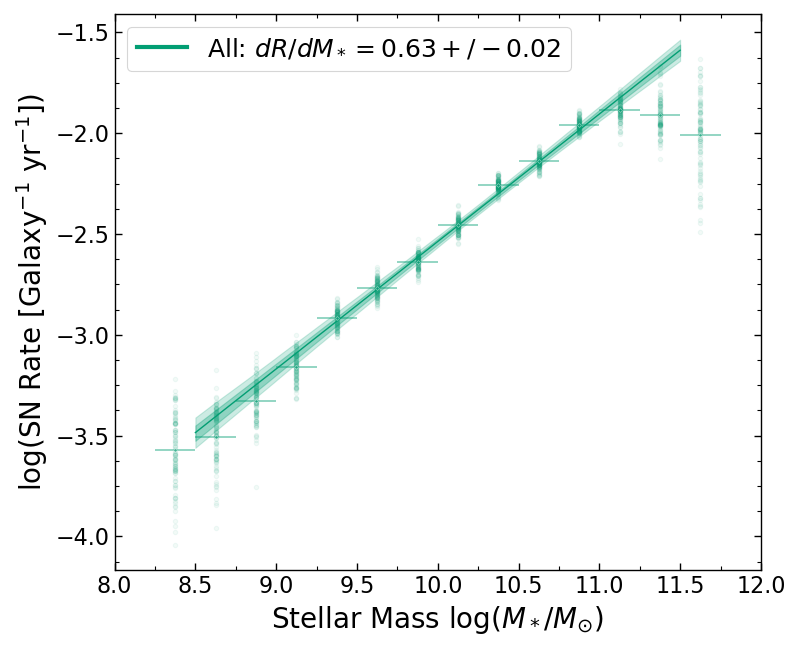
\includegraphics[width=.5\textwidth]{figs/rate_vs_mass_all.png}
    \caption{The rate per galaxy of SNe Ia as a function of stellar mass. Horizontal error bars represent the width of the stellar mass bins. Vertical error bars are estimated via a Monte-Carlo resampling of the rate given the uncertainties in stellar mass. The linear fit is based on all but the lowest and highest mass bins, and takes into account uncertainties in the rate.}%The blue lines indicate the best fitting model based on a $t^{\beta}$ power law DTD convolved with SFHs based on the \citet{Childress2014} model}
    \label{fig:rate_raw}
\end{figure}

\begin{figure}
    \centering
    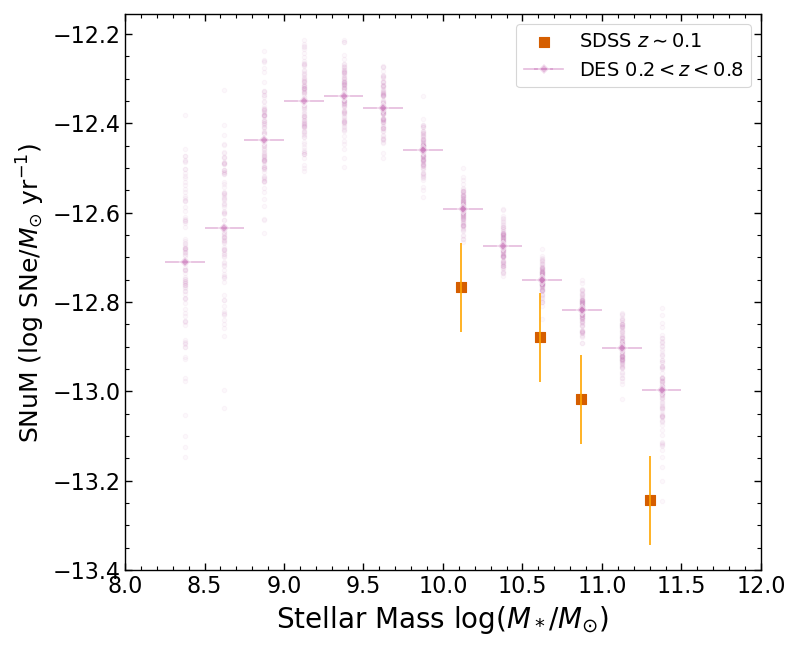
\includegraphics[width=.5\textwidth]{figs/SNuM.png}
    \caption{SN Ia rate per unit stellar mass as function of galaxy stellar mass. Error bars are the same as Fig. \ref{fig:rate_raw}. SDSS data (orange squares) are taken from \citet{Graur2013}. The systematically higher SNuM in DES is likely caused by the higher redshift of the sample. }%The blue lines indicate the best fitting model based on a $t^{\beta}$ power law DTD convolved with SFHs based on the \citet{Childress2014} model}
    \label{fig:snum}
\end{figure}

%\begin{figure}
%    \centering
%    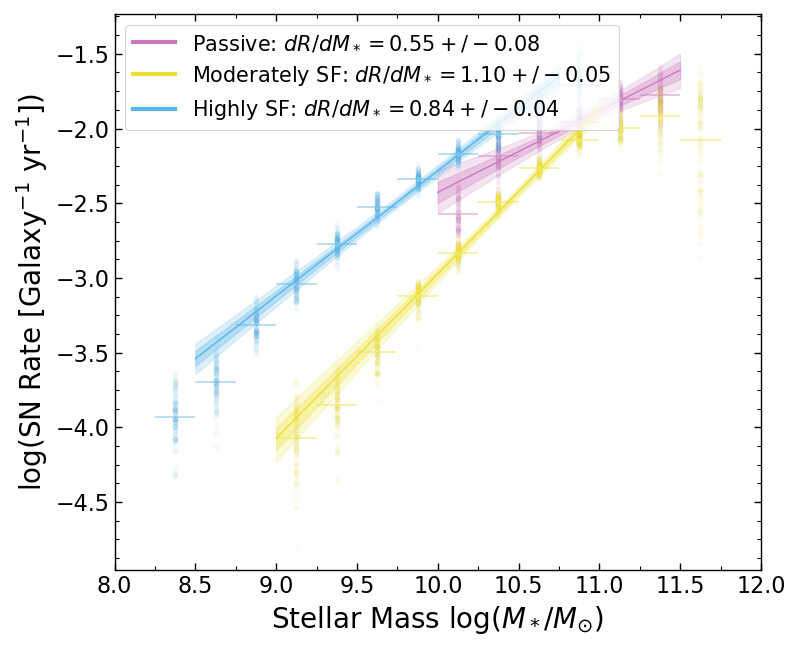
\includegraphics[width=.5\textwidth]{figs/rate_vs_mass_split_sfr.png}
%    \caption{The rate per galaxy of SNe Ia as a function of stellar mass for moderately and highly star-forming galaxies, as well as passive galaxies.}%The blue lines indicate the best fitting model based on a $t^{\beta}$ power law DTD convolved with SFHs based on the \citet{Childress2014} model}
%    \label{fig:rate_raw_split_sfr}
%\end{figure}
%%% MODEL %%%

\begin{figure*}
    \centering
    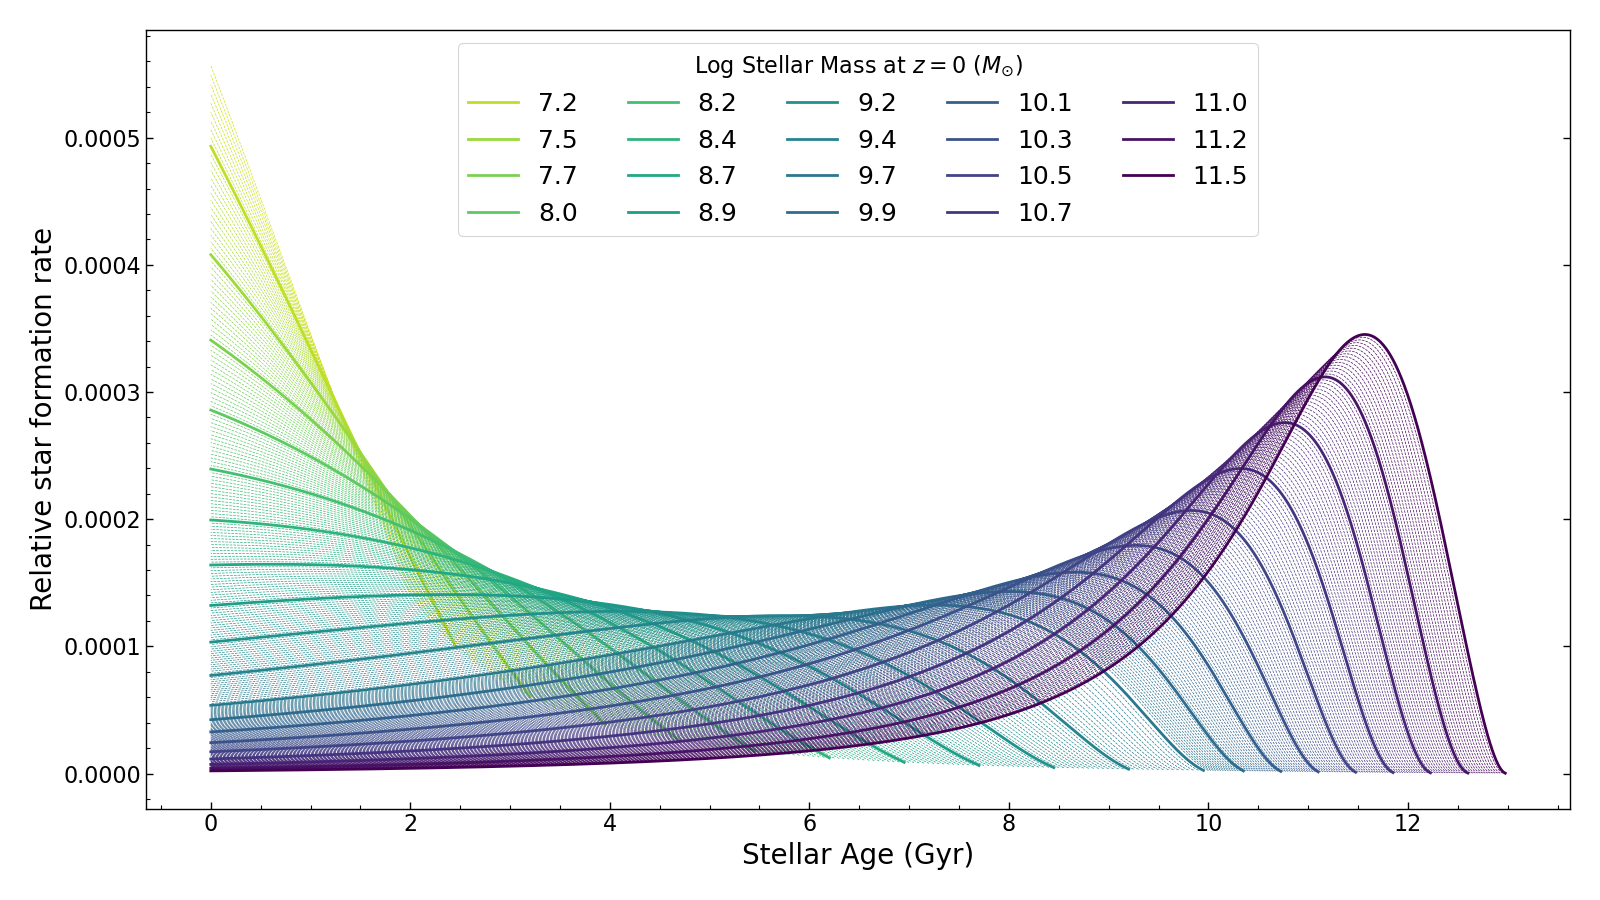
\includegraphics[width=\textwidth]{figs/SFHs_colour.png}
    \caption{The stellar mass assembly of the Universe as prescribed by the toy model of \citet{Childress2014}. Galaxies with high stellar mass at $z=0$ formed the majority of their stars in the distant past, while lower-mass galaxies are still actively star forming in the present day.}
    \label{fig:SFHs}
\end{figure*}

%%%%%% RESULTS %%%%%%%%

\section{The per-galaxy rate of type Ia supernovae}
\label{sec:rates}
The rate of SNe per galaxy ($R_{\mathrm{G}}$) per year in a transient survey can be approximated by the equation:
\begin{equation}
    R_{\mathrm{G}} = \frac{N_{\mathrm{SN}}}{N_{\mathrm{G}}} \frac{V_{\mathrm{G}}}{V_{\mathrm{SN}}}\frac{1}{T_{\mathrm{SN  survey}}}\,,
\label{eq:rate1}
\end{equation}
where $N_{\mathrm{SN}}$ and $N_{\mathrm{G}}$ are the respective number of SNe and galaxies detected, $V_{\mathrm{SN}}$ and $V_{\mathrm{G}}$ the volumes from which the SNe and G samples were taken, and $T$ the duration of the SN survey in years. 

As described in Section \ref{sec:incompleteness}, the values of $N_{\mathrm{SN}}$ and $N_{\mathrm{G}}$ that we observe are underestimates of the true numbers due to observational incompleteness -- we do not detect and count all SNe in the volume $V_{\mathrm{SN}}$, nor do we detect and count all galaxies in the volume $V_{\mathrm{G}}$. We thus estimate the intrinsic numbers of SNe and galaxies by multiplying the observed numbers by their respective incompleteness corrections calculated in Sections \ref{subsec:incompleteness_SNe} and \ref{subsec:incompletenss_SN_hosts} for SNe and Section \ref{subsec:incompleteness_field} for field galaxies:

\begin{equation}
    N_{\mathrm{SN,intrinsic}} = \sum_i^{n_{\mathrm{SN}}}\eta_{\mathrm{SN,}i}\,,
    \label{eq:corr_SN}
\end{equation}
and
\begin{equation}
    N_{\mathrm{G,intrinsic}} = \sum_j^{n_{\mathrm{G}}} \eta_{\mathrm{G,}j} 
    \label{eq:corr_G}
\end{equation}
for each SN $i$ and galaxy $j$.

\begin{figure}
    \centering
    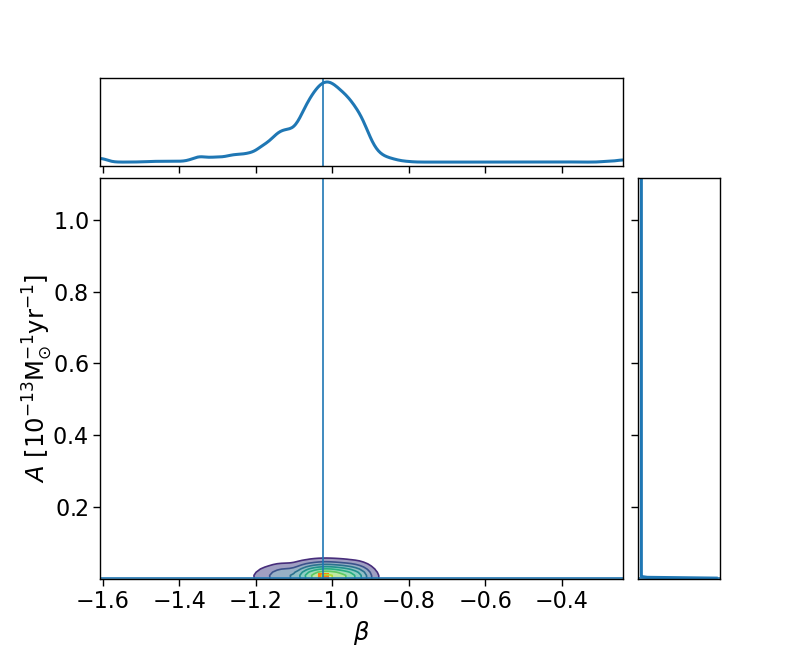
\includegraphics[width=.5\textwidth]{figs/beta_A_Qerf1.1_corner.png}
    \caption{Posterior distributions for DTD slope $\beta$ and normalisation $A$. %The blue lines indicate the best fitting model based on a $t^{\beta}$ power law DTD convolved with SFHs based on the \citet{Childress2014} model}
    \label{fig:corner_beta_norm}}
\end{figure}

\begin{figure}
    \centering
    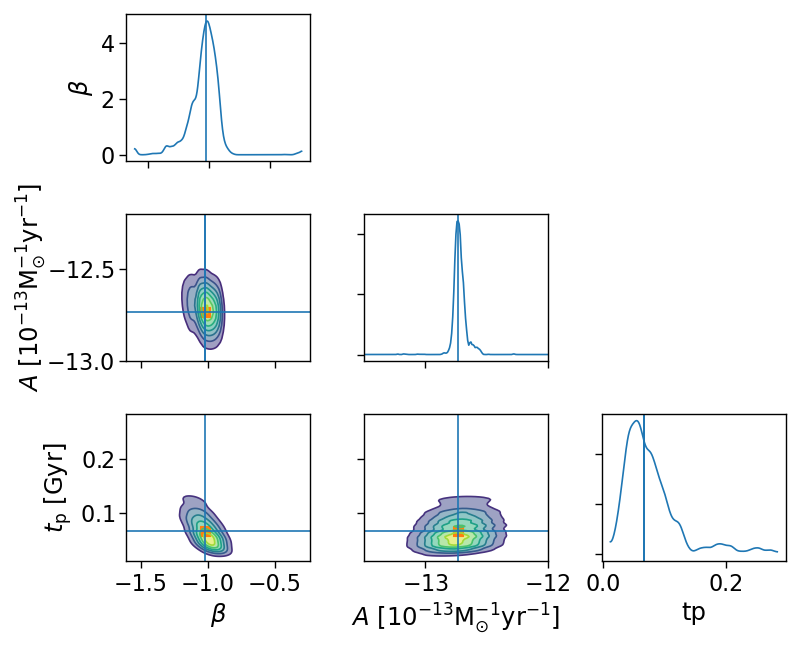
\includegraphics[width=.5\textwidth]{figs/beta_A_tp_Qerf1.1_corner.png}
    \caption{Posterior distributions for DTD parameters $\beta$, $A$, and $t_{\mathrm{p}}$. \textbf{This needs updating once final chains are run. Axes labels need sorting.} %The blue lines indicate the best fitting model based on a $t^{\beta}$ power law DTD convolved with SFHs based on the \citet{Childress2014} model}
    \label{fig:corner_beta_norm_tp}}
\end{figure}


\begin{figure}
    \centering
    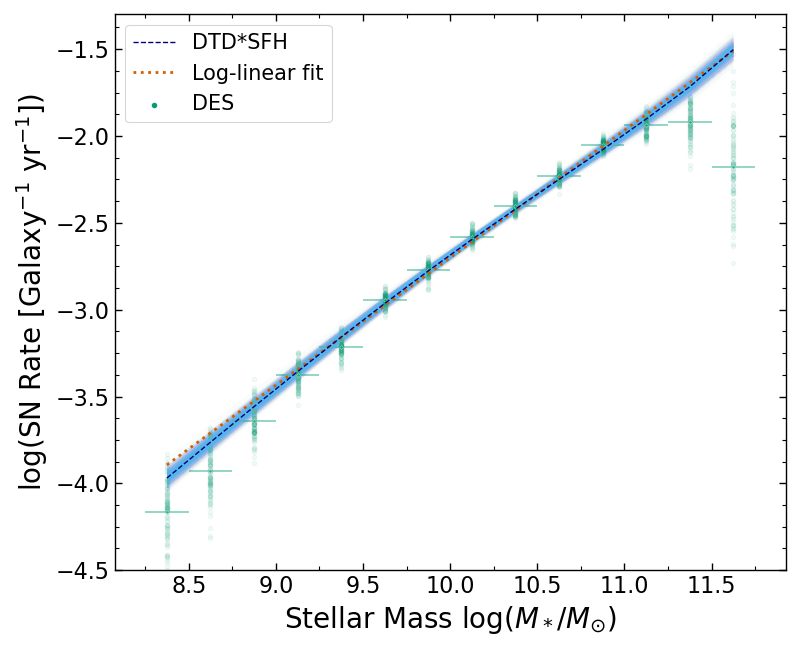
\includegraphics[width=.5\textwidth]{figs/rate_vs_mass_DTD_fit_beta_norm_Qerf1.1.png}
    \caption{Rate per galaxy of SNe Ia as a function of stellar mass (green points) along with the prediction from the best fitting DTD parameters $\beta$, $A$, and $t_{\mathrm{p}}$ forward modelled through Eq. \ref{eq:galaxy_rate}. Samples from the posterior distribution of the model log rate are drawn in cyan while the black dashed line is the mean of the posterior.%The blue lines indicate the best fitting model based on a $t^{\beta}$ power law DTD convolved with SFHs based on the \citet{Childress2014} model}
    \label{fig:rate_fitted}}
\end{figure}

By binning both the SN hosts and field galaxies by their stellar mass we measure the mean SN Ia rate per galaxy as a function of stellar mass, $R_{\mathrm{G}}(M_*)$. We employ a bootstrap Monte-Carlo approach in order to estimate the uncertainty in the value of the rate in each stellar mass bin. The probability distribution function (PDF) of each galaxy's stellar mass is represented by the sum of two half Gaussian distributions to represent the asymmetric positive and negative uncertainties derived in the SED fitting stage (Section \ref{sec:data}). For each SN host and field galaxy, we take 100 samples of its stellar mass by drawing at random from its PDF. For each of the 100 samples we calculate the SN rate per galaxy in each stellar mass bin via Eq \ref{eq:rate1}, using the completeness-corrected values of $N_{\mathrm{SN}}$ and $N_{\mathrm{SN}}$ from Eqs. \ref{eq:corr_SN} and \ref{eq:corr_G} respectively. 

The rate of SNe Ia per galaxy as a function of stellar mass is shown in Fig. \ref{fig:rate_raw}. The relationship between SN Ia rate and galaxy stellar mass is well described by a linear function in log space, which corresponds to a power law. To find the slope and intercept that best describe the data we use Bayesian inference. To sample the posterior we use the enhanced no-U-turn Sampler (NUTS) algorithm \citep{Betancourt2017}, which is a variant of Hamiltonian Monte-Carlo (HMC), implemented in the Stan programming language \citep{Carpenter2017}. We describe the fitting procedure in full detail in Appendix \ref{appendix:linear_fits}. We measure a slope of $0.70\pm0.02$, which is broadly consistent with the values found in SNLS and SDSS by \citet{Sullivan2006} and \citet{Smith2012} respectively. It is evident that the linear fit is not consistent with the data across the full range of stellar mass considered. In particular, there appear to be two locations of interest: firstly, the slope is steeper at masses lower than $10^9$ M$_{\odot}$; secondly there is an apparent flattening and possibly a turnover at masses around and above $10^{11}$ M$_{\odot}$. The most likely cause of these divergences is because the SN rate is driven by the SFH which is not a linear function of stellar mass (see Section \ref{sec:model}). Second order effects may also be important, and we address these in the following sections.

\subsection{Rate per unit stellar mass \label{subsec:snum}}
\textbf{short section showing SNUM and how it matches past results}

\section{Modelling the per-galaxy rate of type Ia supernovae}
 \label{sec:model}
 
In Section \ref{sec:rates} and Fig. \ref{fig:rate_raw} we showed that the SN Ia rate per galaxy as a function of stellar mass is approximated by, but not perfectly described by, a power-law (and thus a linear relationship in log space). In this section, we introduce a physical model in order to better fit the observed rate vs stellar mass relationship. 

We begin by considering the delay time distribution of SNe Ia.
We represent the SN Ia DTD by a power law, which we consider effective after some "prompt time" $t_{\mathrm{p}}$, before which its value is set to 0. This is generally interpreted as the time taken for WDs to form after the burst of star formation. The DTD is thus:
\begin{equation}
 \Phi(\tau) = \left\{
    \begin{array}{@{}cc@{}}
    0 , & \tau < t_{\mathrm{p}} \\
    A\left(\frac{\tau}{\mathrm{Gyr}}\right)^{\beta} , & \tau \geq t_{\mathrm{p}}
    \end{array}\right.
        \label{eq:dtd}
\end{equation} 
where $\tau$ is the time since a burst of star formation, and $A$ is a normalisation at $\tau=1$ Gyr. If all stars in a galaxy were formed at a single epoch $t_f$, the DTD would describe the rate of SNe at an observation time $\tau = t_0$. However in reality galaxies are formed by the gradual build up of stellar mass over several epochs of star formation -- the distribution of this mass build up is known as the star-formation history (SFH). The rate of SNe Ia is thus the sum of the DTD evaluated for each epoch of star formation, multiplied by the stellar mass formed in that epoch. Mathematically this is represented by the convolution of the DTD and SFH:
 
\begin{equation}
    R_{\mathrm{G}} = \int_{t_0}^{\infty} \psi(t_0-\tau)\Phi(\tau)\,d\tau \,,
    \label{eq:galaxy_rate}
\end{equation}
where $t_0$ is the epoch at which the galaxy is observed, and $\psi$ is the SFH. 

In previous work \citep[e.g.][]{Strolger2004,Maoz2012} it has been common to determine the SFH for every galaxy in the survey via SED fitting. Eq. \ref{eq:galaxy_rate} is then used to calculate an expected number of SNe in each galaxy given the effective survey time, which is compared to the observed number in that galaxy (usually 0 and occasionally 1) using Poisson statistics. This method relies on either photometry covering several wavelength bands, or optical spectra with high signal-to-noise ratio (S/N), in order to distinguish accurately between SFHs. Such accuracy is not possible for the DES sample: we do not possess spectra of all galaxies in the field, and in some cases only have the four optical bands available -- and have a maximum of eight from NUV to NIR -- from which to infer a SFH. This lack of detail is compounded by our relying on photometric redshifts which add an extra layer of uncertainty to the calculation. 

Instead of determining individual SFHs for each galaxy in our field sample, we use an empirical approach to estimate mean SFHs for galaxies as a function of their stellar mass at any given redshift (or equivalently, time $t_0$), that can be represented as $\hat \psi \left(t_0 -\tau; M_* \right)$. This method paves the way for modelling the SN Ia rate as a function of stellar mass by combining the mean SFHs and the DTD through Eq. \ref{eq:galaxy_rate}, and thus placing constraints on the DTD.

\subsection{Modelling the star formation histories of galaxies \label{subsec:method_sfh}}

To model the SFH of galaxies as a function of their stellar mass we adopt the prescription of stellar mass assembly of \citet{Childress2014}, which draws on the work of \citet{Zahid2012}. In the model, galaxies are expected to evolve smoothly along the so-called "main sequence of star formation" whereby the SFR of a galaxy of stellar mass $M_*$ at redshift $z$ is determined by a simple relationship (the SMz relation, \citealt{Zahid2012}). Specifically, we implement their "fine-tuned" model (C14 Eq. A7), whereby the SMz flattens above $z\sim2$ in line with observations \citep{Stark2013}. We adjust this model slightly and arrive at a final SMz:

\begin{equation}
    \Psi(M_*,z) = \left(\frac{M_*}{10^{10}}\right)^{0.7}\frac{\exp{\left(1.9z\right)}}{\exp{\left(1.7\left(z-2\right)\right)} + \exp{\left(0.2\left(z-2\right)\right)} } [\mathrm{M}_{\odot} \mathrm{yr}^{-1}]\,.
\end{equation}

As galaxies grow, their SFR begins to slow down and eventually shut off almost entirely in a process known as quenching. We adopt the quenching penalty $p_Q$ directly from \citet{Childress2014}:
\begin{equation}
    p_Q(M_*,z) = \frac{1}{2}\left[1 - \mathrm{erf}\left(\frac{\log(M_*) - \log(M_Q(z))}{\sigma_Q}\right)\right]\,,
    \label{eq:pq}
\end{equation}
where $M_Q(z)$ describes how the quenching mass evolves with redshift, and $\sigma_Q$ is the transition scale which controls how fast a galaxy quenches. We adopt the observationally motivated form of the quenching mass evolution (Eq. A8 from \citealt{Childress2014}):
\begin{equation}
    \log(M_q(z)/\mathrm{M}_{\odot}) = 10.077 + 0.636z \,, 
    \label{eq:mq}
\end{equation}
and a transition scale of $\sigma_Q = 1.1$ which provides a good fit to data from the Galaxy And Mass Assembly (GAMA) survey \citep{Baldry2012}.

As per \citet{Childress2014} we plant seed galaxies with initial masses of $10^6 \mathrm{M}_{\odot}$ at intervals of 50 Myr for look-back times $1 \leq t_f \leq 10$ Gyr, and 25 Myr for look-back times $10 \leq t_f \leq 13$ Gyr, and evaluate the model with a time step of 0.5 Myr.

The result of our toy model is shown in Fig. \ref{fig:SFHs}. Galaxies with high masses at $z=0$ formed the vast majority of their stars in the first few Gyr and are now likely to be passive with old stellar populations, while low-mass galaxies are currently strongly star-forming with a vast majority of young stars. Galaxies with masses around $10^{10} \mathrm{M}_{\odot}$ are composed of a mixture of young and older stellar populations.

\textbf{Add plot showing that the toy model recreates the stellar mass function?}

%\textbf{TEMPTED TO DITCH THIS SINCE OUR SFR IS SKETCHY}
%In order to make a more detailed comparison of our results with those of \citet{Sullivan2006} and \citet{Smith2012}, we split galaxies according to their sSFR: galaxies with sSFR$\leq -11.5$ yr$^{-1}$ are denoted as passive, those with $-11.5 < \mathrm{sSFR} \leq -9.5$ are moderately star-forming, and those with sSFR $>-9.5$ are labelled as highly star-forming. The results when split this way are shown in Fig. \ref{fig:rate_raw_split_sfr}. Star-forming galaxies show a steeper slope than their passive counterparts, with values of $1.10 \pm 0.05$ and $0.84 \pm 0.04$ for moderate and highly star-forming galaxies respectively, while passive galaxies show a much shallower slope of $0.55 \pm 0.08$. These values are broadly similar to those measured in SDSS by \citet{Smith2012}, with star-forming galaxies showing steeper slopes than passives (\citet{Smith2012} found 1.01 and 0.72 for SF and passive, respectively). We note that we detect no passive galaxies with mass below $10^{10} \mathrm{M}_{\odot}$. Above this value, the \citet{Smith2012} data for passive galaxies is considerably flatter than that which we measure. On the other hand our results are inconsistent with those found at a similar redshift to the DES data in SLNS \citep{Sullivan2006}, who measured a slope of 1.10 in passives but 0.66 and 0.74 in moderate and highly star-forming galaxies respectively. We note that the moderately star-forming slope is thus consistent between DES and SNLS, but the slopes of passive and highly star-forming galaxies are swapped.
\renewcommand{\arraystretch}{1.2}
\begin{table}
	\centering
	\caption{Results of the Bayesian parameter estimation for the SN Ia DTD.}
	\label{tab:dtd_results}
	\begin{tabular}{lccr} % four columns, alignment for each
		\hline
		 &$\beta$ & $A$ & $t_{\mathrm{p}}$\\
		 &-       & $10^{-13}$ M$_{\odot}^{-1}$yr$^{-1}$ & Gyr \\
		\hline
		Fixed $t_{\mathrm{p}}$ & $-0.97_{-0.05}^{+0.05}$ &  $1.73_{-0.05}^{+0.05}$ & -\\
		Free $t_{\mathrm{p}}$ & $-1.02 _{-0.11} ^{+0.08}$ & $1.86 _{-0.13} ^{+0.19}$ & $0.067 _{-0.023} ^{+0.043}$\\
		Fixed $A$, $\beta$ & - & - & $0.047_{-0.007}^{+0.008}$\\
		\hline
	\end{tabular}
\end{table}

\subsection{Constraints on the SN Ia delay time distribution}
\label{subsec:results_dtd}

At the beginning of this Section, we showed how the rate of SNe Ia is driven by the convolution of the SFH of galaxies and the SN Ia DTD (Eq. \ref{eq:galaxy_rate}). We then prescribed a model to infer the mean SFHs of galaxies of any given stellar mass. Here, we measure the DTD by forward modelling it through Eq. \ref{eq:galaxy_rate} at the stellar masses corresponding to the centres of the bins in Fig. \ref{fig:rate_raw}. 

We assume a DTD $\Phi(\tau)$ with a power-law form described by index $\beta$ (Eq. \ref{eq:dtd}), normalisation $A$ and effective after prompt time $t_{\mathrm{p}}$. As per Section \ref{sec:rates}, we constrain the parameters via Bayesian inference, using HMC. At each step of the sampling procedure the model is re-calculated via Eq. \ref{eq:galaxy_rate}, and evaluate the likelihood assuming that the rate data are normally distributed about their means. For $\beta$ we adopt a Gaussian prior with hyper-parameters $p(\beta) \sim \mathcal{N}(-1\,,0.3)$. We fit for $A$ in log space, and adopt a Gaussian prior (in log space) with hyper-parameters $p(A) \sim \mathcal{N}(-12.7\,, 0.5)$.

SNe Ia do not occur instantaneously after an episode of star formation. Instead stars with zero-age main-sequence (ZAMS) masses less than $8~\mathrm{M}_{\odot}$ take time to evolve along the main sequence and form WDs and this time is not well constrained. In many works this ``prompt time" which we denote $t_{\mathrm{p}}$ is fixed to some value expected to be the minimum time for a star to evolve off the MS and become a WD, such as 40~Myr \citep{Maoz2012,Graur2013,Graur2014}. Other studies have left $t_{\mathrm{p}}$ as a free parameter \citep{Heringer2019,Castrillo2020}. We perform three fits: one with $t_{\mathrm{p}}$ fixed at 40 Myr, one with it as a free parameter along with $\beta$ and $A$, and a third with $\beta$ and $A$ fixed and  $t_{\mathrm{p}}$ free. We fit $t_{\mathrm{p}}$ in log space and adopt a Gaussian prior with hyper-parameters $p(\log(t_{\mathrm{p}})) \sim \mathcal{N}(-1.3\,,0.2)$, which corresponds to being centred around 50~Myr. Choosing this regime to fit allows more prior weight to be placed on shorter prompt times as per the majority of the literature. 

The posterior distributions for the fit parameters are found in Figs. \ref{fig:corner_beta_norm} and \ref{fig:corner_beta_norm_tp} for the fixed and free $t_{\mathrm{p}}$ fits respectively, and the posterior means and standard deviations are summarised in Table \ref{tab:dtd_results}. In Fig. \ref{fig:rate_fitted} we show the SN rate per galaxy predicted by the model assuming the best fitting DTD parameters from Table \ref{tab:dtd_results} compared to the data as presented in Section \ref{sec:rates}. The model provides a good fit across a wide range of stellar mass. The model clearly diverges from the simple log-linear fit, describing better the suppressed rate at the low and high ends of the stellar mass range, as well as the enhanced rate around $10^{10}$ M$_{\odot}$. This improvement provides evidence to support the DTD*SFH model. However, the model prediction still diverges from the data at high ($>10^{11.25}$ M$_{\odot}$), suggesting that these data cannot be explained by the our model, but are driven by further processes that we have not included. We discuss these in Section \ref{subsec:discussion}.

\subsection{Comparison to previous DTD measurements \label{subsec:compare_dtd}}

\subsubsection{The DTD power law index \label{subsubsec:compare_beta}}
We measure a DTD power law index of $-1.14\pm0.05$. This value is consistent with the majority of previous analyses using various methods. Our measurement provides an independent support to the values close to $-1$ found using volumetric rates \citep[e.g.][]{Graur2013,Frohmaier2019}, individual galaxy SFHs \citep[e.g.][]{Maoz2012,Graur2013}, and galaxy clusters \citep[e.g.][]{Maoz2010} although our slope is marginally inconsistent with that of \citet{Heringer2019}. 

\subsubsection{The DTD normalisation \label{subsubsec:compare_A}}
We measure a DTD normalisation (i.e. the rate of SNe 1 Gyr after star-formation) of $1.73 \pm 0.05 \times 10^{-13}$~M$_{\odot}^{-1}$~yr$^{-1}$. \citet{Graur2013} found a value of $7 \times 10^{-14}$~M$_{\odot}^{-1}$~yr$^{-1}$ using the SFH technique, whereas \citet{Heringer2019} report $7 \times 10^{-13}$~M$_{\odot}^{-1}$~yr$^{-1}$. These results lie either side of our measured value. \citet{Heringer2019} note that the normalisation recovered from the SFHR method is sensitive to the assumed prompt time $t_{\mathrm{p}}$, a degeneracy that is also apparent our method. 

By integrating the normalised DTD over cosmic time, we obtain an estimate of the average SN Ia efficiency $N_{\mathrm{Ia}}/M_*$ which represents the number of SNe Ia formed per unit mass of stars formed. We measure $N_{\mathrm{Ia}}/M_* = 2.0~_{-1.6}^{+5.0} \times 10^{-3}~\mathrm{SNe}~\mathrm{M}_{\odot}^{-1}$. 



\subsubsection{The SN Ia prompt time \label{subsubsec:compare_tp}}

The majority of works in the field have constrained the DTD power-law slope, and many also estimate its normalisation. Conversely, few have attempted to constrain the time after a burst of star-formation at which SNe Ia begin to explode -- the prompt time $t_{\mathrm{p}}$. In most cases, $t_{\mathrm{p}}$ has been fixed at some fiducial value such as 40~Myr, which is derived from the lifetime of 8~M$_{\odot}$ stars. \citet{Castrillo2020} included $t_{\mathrm{p}}$ (which they denote $\Delta$) in their fit, and find a value of $50_{-35}^{+100}$~Myr which is consistent with both 40~Myr as well as our best fitting value of $67_{-23}^{+43}$~Myr for the three-parameter fit and $47_{-7}^{+8}$~Myr with $\beta$ and $A$ fixed. \citet{Heringer2019} also present fits with varying prompt times, although they don't fit for the parameter itself. They find that varying $t_{\mathrm{p}}$ changes the recovered normalisation, which is consistent with the degeneracy seen in our results (Fig. \ref{fig:corner_beta_norm_tp}). Overall, we find results for $t_{\mathrm{p}}$ that are consistent with the fiducial value of 40~Myr and adopt this value for the remainder of the analysis.

\begin{figure}
    \centering
    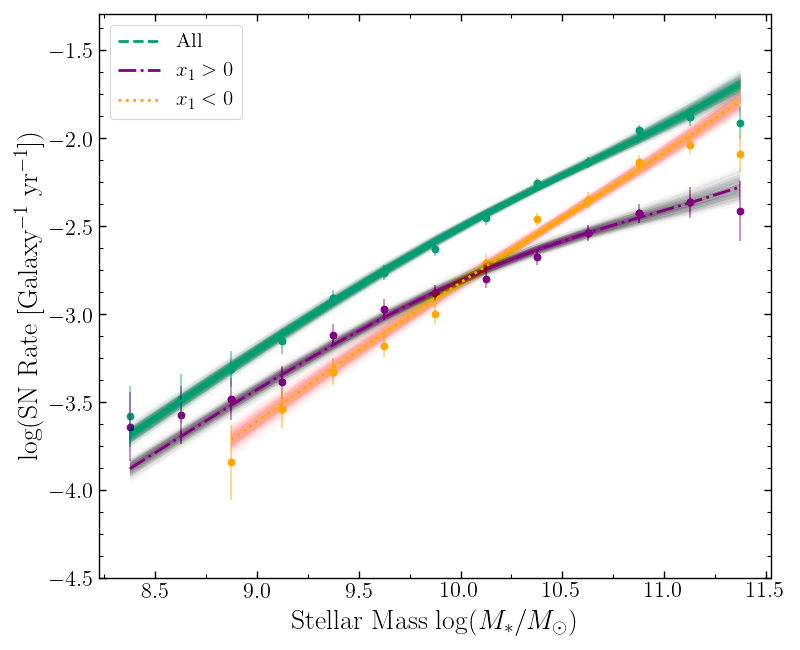
\includegraphics[width=.5\textwidth]{figs/rate_vs_mass_DTD_fit_beta_norm_Qerf1.1_split_x1.png}
    \caption{As per Fig. \ref{fig:rate_fitted} but with the data split by their stretch parameter $x_1$.%The blue lines indicate the best fitting model based on a $t^{\beta}$ power law DTD convolved with SFHs based on the \citet{Childress2014} model}
    \label{fig:rate_fitted_split_x1}}
\end{figure}


\begin{figure}
    \centering
    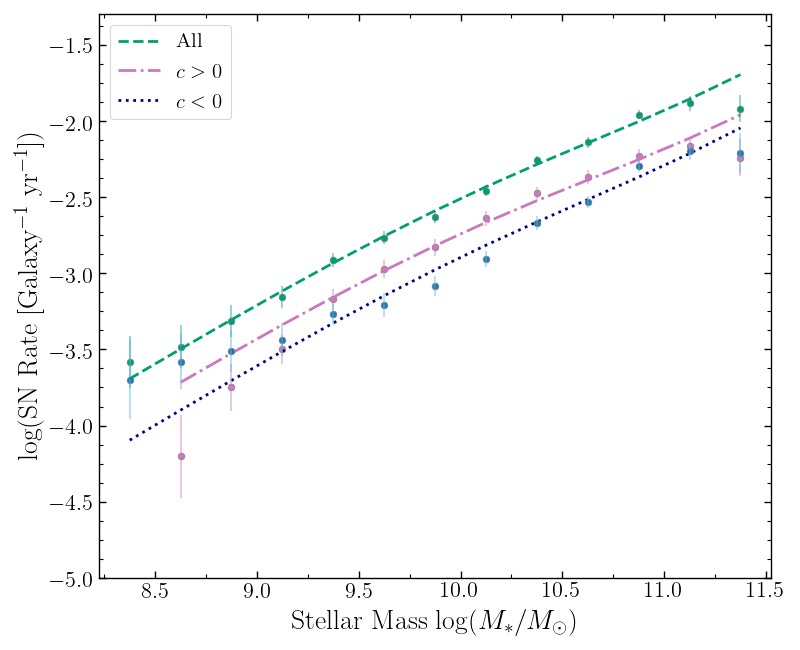
\includegraphics[width=.5\textwidth]{figs/rate_vs_mass_DTD_fit_beta_norm_Qerf1.1_split_c.png}
    \caption{As per Fig. \ref{fig:rate_fitted} but with the data split by their colour parameter $c$.%The blue lines indicate the best fitting model based on a $t^{\beta}$ power law DTD convolved with SFHs based on the \citet{Childress2014} model}
    \label{fig:rate_fitted_split_c}}
\end{figure}

\renewcommand{\arraystretch}{1.2}
\begin{table}
	\centering
	\caption{Results of the Bayesian parameter estimation for the SN Ia DTD.}
	\label{tab:dtd_results_split_lc}
	\begin{tabular}{crr} % four columns, alignment for each
		\hline
		 Sample &$\beta$ & $A$ \\
		 &-       & $10^{-13}$ M$_{\odot}^{-1}$yr$^{-1}$ \\
		\hline
		Fiducial & $-1.18\pm0.09$ &  $1.16\pm0.08$ \\
	    $x_1 < 0$ & $-0.79\pm0.08$ &  $1.19 \pm0.05$ \\
		$x_1 > 0$ & $-1.68 _{ -0.15} ^{ +0.14}$ & $0.51\pm0.12$ \\
		$c < 0$ & $-1.09 _{ -0.07} ^{ +0.08}$ & $0.89\pm0.04$ \\
		$c > 0$ & $-1.19\pm0.09$ & $1.16\pm0.08$ \\
		\hline
	\end{tabular}
\end{table}
\subsection{Second order processes affecting the supernova rate \label{subsec:discussion}}

The use of SN Ia rate measurements to constrain the SN Ia DTD has consistently led to a $t^{-1}$ power-law, which is widely accepted as evidence supporting the DD scenario. While our results are also consistent with those derived in previous studies, our model is mildly inconsistent with the SN rate per galaxy at very high stellar mass. The model over predicts the observed rate of SNe Ia in galaxies in that stellar mass range, caused either by a miscalculation of the rate or second order effects acting to suppress the rate compared to the fiducial model.

\subsubsection{Stochasticity of galaxy evolution}

The toy model of stellar mass assembly used in this work includes several assumptions about the evolution of galaxies. In particular, it is assumed that galaxies evolve independent of each other, growing up the SFMS until they reach a mass at which they quench and star formation ceases. While these simplifications describe the average properties of galaxies well \citep{Zahid2012, Childress2014}, they struggle to describe the more stochastic nature of galaxy evolution that occurs at the low and high mass ends: starbursts and quenching episodes, respectively. 

At some point along the evolutionary pathway, galaxies begin to cease star formation due to a combination of processes that together are known as quenching. In our model of mass assembly the characteristic mass at which quenching occurs is described by Eq. \ref{eq:mq}, and the rate of the transition from star forming to passive (as a function of the stellar mass) is determined by the transition scale $\sigma_{\mathrm{Q}}$ which we set to 1.1 based on GAMA observations. It is possible that this transition is too narrow and that quenching happens too fast in our model, leading to an under-prediction of the prompt fraction of SNe in the highest mass galaxies. To address this issue we rerun the mass assembly model with $\sigma_{\mathrm{Q}} = 1.5$ as per the nominal analysis of \citet{Childress2014} and refit the SN Ia rate data. We find that the adapted quenching model does not change the ability of the model to adequately fit the high-mass turnover in the SN rate.

\subsubsection{Effects of stellar metallicity}

One possible cause of the discrepant SN Ia rate at high stellar mass is the effect of stellar metallicity. Metallicity has been previously invoked to explain irregularities or divergences from the fiducial DTD \citep[e.g.][]{Strolger2010,Meng2011,Kistler2013}. Metallicity may affect the observed rate of SNe in two ways: firstly, it can affect the time taken for a star to evolve along the main sequence ($t_{\mathrm{MS}}$) -- Stellar metallicity has varying effects on the MS lifetime of stars \citep[e.g.][]{Georgy2013,Amard2020}, which is also dependent upon initial rotation and degree of mixing; secondly it can affect the time taken from WD formation to SN Ia explosion -- low metallicity stars should produce higher-mass WDs \citep[e.g.][]{Umeda1999,Marigo2007}, resulting in a higher SN Ia rate \citep{Kistler2013}. 

The mass-metallicity relation (MZR) is a strong observed correlation between galaxy stellar mass and gas-phase metallicity \citep[e.g.][]{Tremonti2004}, whereby higher mass galaxies have undergone more cycles of stellar evolution and have been polluted with heavy elements created in stars and released in SNe. Thus, the mass of a host galaxy is inextricably linked to the metallicity of its hot gas. However, the nature of the DTD complicates matters, since stars of different ages were formed at different epochs where the galaxy had a different stellar mass and thus different metallicity. Therefore, there is not a direct correlation between the metallicity of SN Ia progenitors and their observed host galaxy stellar mass.  This caveat notwithstanding, it may be an expected consequence of the stipulations of e.g. \citet{Kistler2013} that the rate of SNe Ia is suppressed in the highest mass galaxies where the metallicity is highest, as is the case in our data.

\section{The delay-time distribution as a function of supernova properties}
\label{sec:split_x1_c}

In the previous sections we have considered all SNe that passed the various quality, standardisation, and redshift cuts. However, it is well established that SNe Ia show correlations of varying strength between properties of their light curves and host galaxies. For example, measures of the light curve duration (e.g. decline rate $\Delta m_{15}$, or stretch such as SALT2 $x_1$) are known to correlate with host galaxy properties such as stellar mass \citep{Lampeitl2010,Sullivan2010} and specific SFR \citep{Rigault2018}. In this section we split the DES SNe Ia by their colour and stretch and assess how the measured rates and DTDs vary across this parameter space. To do so we split the sample into sub-samples with $x_1 = 0$ and $c=0$ as the divisions points respectively. We repeat the analyses of Sections \ref{sec:rates} and \ref{sec:model}, performing the DTD fitting with a fixed $t_{\mathrm{p}} = 40$~Myr, and present the results in Table \ref{tab:dtd_results_split_lc}.

\subsection{Splitting by SN stretch \label{subsec:split_x1}}

The SN Ia rate as a function of stellar mass SNe split by stretch is shown in Fig. \ref{fig:rate_fitted_split_x1}. The evolution of the rate with stellar mass is significantly different for the two sub-samples: high-stretch SNe dominate the rate at low stellar mass but tail off in the higher mass galaxies, while low-stretch SNe are subdominant in low mass galaxies but display a much steeper dependence on stellar mass and make up the vast majority of SNe in high-mass hosts. These measurements reflect the observed correlations of $x_1$ with stellar mass and sSFR. The corresponding DTD fit results in a steep power-law for high-stretch SNe indicative of a population of predominantly prompt SNe, and a much shallower decay slope for low-stretch SNe representing a much more delayed population. Such a distinction has been predicted by \citet{Rigault2013,Childress2014,Rigault2018,Nicolas2020} based on the intrinsic $x_1$ distribution and its observed relationship with stellar mass and age.

From the differing DTDs that describe SNe with low and high stretch values we infer that there are either multiple channels through which SN Ia explode which occur on differing timescales, or that the explosion mechanism evolves with progenitor age. Two scenarios, that are not necessarily mutually exclusive, that could lead to different DTD decay rates are as follows. 
The first such scenario is to assume that all SNe Ia come from the same initial population of stars, and thus that the progenitors of both low and high stretch SNe form at the same time. It is then necessary to invoke models in which the WD progenitors of low-stretch SNe evolve on longer timescales than those of high-stretch SNe, for example due to a different initial binary separation distribution or accretion rate.

Alternatively, low- and high-stretch SNe could form via identical evolutionary channels but with a different onset time since the episode of star-formation. The predominantly high-stretch "prompt" SNe would begin exploding as soon as the WDs are formed (nominally 40 Myr) whereas the mainly low-stretch "tardy" SNe would only begin exploding after an extended period of time of the order 1 Gyr. The rates of both populations would then both follow the fiducial $t^{-1}$ distribution beginning at this onset time.
Such a scenario has been explored theoretically, primarily in the sub-Chandrasekhar mass (sub-$M_{\mathrm{Ch}}$) paradigm \citep[e.g.][]{Sim2010,Blondin2017,Shen2017}, usually associated with various forms of the DD scenario. Sub-$M_{\mathrm{Ch}}$ SNe Ia typically involve the merger of two WDs where the SN luminosity is correlated with the mass of the primary WD; a correlation between primary WD mass and age would then lead to the different rates, and apparent DTDs, of low and high-stretch SNe observed in this work. 

We explore this scenario by fitting the stretch-separated sub-samples with modified DTDs. We fix the DTD to a power-law with index $-1$, and fix the normalisation to the best fitting value from the full sample. We model the DTD as comprising two components: the prompt, high-stretch SNe and the tardy, low stretch SNe, and we introduce two timescales, $t_1$ and $t_2$. At $\tau\leq t_1$, the DTD is caused solely by prompt SNe; at $\tau \geq t_2$ only tardy SNe explode. In between where $t_1 \leq\tau\leq t_2$, the DTD is a sum of DTD (prompt) and DTD (tardy), where we model the relative fraction $f$ as a smooth linear slope between $t_1$ and $t_2$:
\begin{equation}
    f_{\mathrm{tardy}} = \frac{\tau - t_1}{t_2 - t_1}\,,
\end{equation}
and
\begin{equation}
    f_{\mathrm{prompt}} = 1 - f_{\mathrm{tardy}}\,.
\end{equation}
With $\beta$ and $A$ fixed,  we fit the split-$x_1$ SN Ia rate with $t_1$ and $t_2$ as free parameters, and weak normal priors $p(t_1) \sim \mathcal{N}\left(0.5~\mathrm{Gyr}, 0.5~\mathrm{Gyr}\right)$ $p(t_2) \sim \mathcal{N}\left(1~\mathrm{Gyr}, 0.5~\mathrm{Gyr}\right)$ and the constraint $t_2 > t_1$.

\subsubsection{The late end of the DTD \label{subsubsec:subtypes}}

Despite the reasonable fit of the evolving population model, the fit to tardy SNe diverges from the data at high stellar mass, corresponding to the oldest average stellar age. It is difficult to reconcile this turnover with the simple DTD models used thus far in this work, as it would require a steepening or complete turn-off of the DTD at late ($\tau\gtrsim 5$~Gyr) times. Here we describe two possible ways in which the model can be reconciled with the data in the highest-mass galaxies.

One possibility is that sub-luminous SNe are more numerous in such predominantly old stellar populations, such that the fraction passing our light curve cuts is lower than the rest of the sample. Such a phenomenon could be caused by SN Ia sub-classes such as SN 1991bg-like SNe, which are known to explode exclusively in old environments \citep{Perets2010} at large delay times $>6$~Gyr \citep{Panther2019}. 



\section{Conclusions}
\label{sec:conclusion}
The last numbered section should briefly summarise what has been done, and describe
the final conclusions which the authors draw from their work.

\section*{Software}

All software used in this publication is publicly available. In particular, we made extensive use of \texttt{numpy} \citep{Harris2020}, \texttt{Astropy} \citep{AstropyCollaboration2013,AstropyCollaboration2018}, \texttt{matplotlib} \citep{Hunter2007}, \texttt{SciPy} \citep{Virtanen2020}, \texttt{pandas} \citep{Mckinney2010}, \texttt{Stan} \citep{Carpenter2017}, \texttt{seaborn} \citep{Waskom2020}, and \texttt{arviz} \citep{Kumar2019}.

\section*{Acknowledgements}

The Acknowledgements section is not numbered. Here you can thank helpful
colleagues, acknowledge funding agencies, telescopes and facilities used etc.
Try to keep it short.

%%%%%%%%%%%%%%%%%%%%%%%%%%%%%%%%%%%%%%%%%%%%%%%%%%
\section*{Data Availability}

 
The inclusion of a Data Availability Statement is a requirement for articles published in MNRAS. Data Availability Statements provide a standardised format for readers to understand the availability of data underlying the research results described in the article. The statement may refer to original data generated in the course of the study or to third-party data analysed in the article. The statement should describe and provide means of access, where possible, by linking to the data or providing the required accession numbers for the relevant databases or DOIs.



%%%%%%%%%%%%%%%%%%%% REFERENCES %%%%%%%%%%%%%%%%%%

% The best way to enter references is to use BibTeX:

\bibliographystyle{mnras}
\bibliography{PhilMendeley} % if your bibtex file is called example.bib


% Alternatively you could enter them by hand, like this:
% This method is tedious and prone to error if you have lots of references
%\begin{thebibliography}{99}
%\bibitem[\protect\citeauthoryear{Author}{2012}]{Author2012}
%Author A.~N., 2013, Journal of Improbable Astronomy, 1, 1
%\bibitem[\protect\citeauthoryear{Others}{2013}]{Others2013}
%Others S., 2012, Journal of Interesting Stuff, 17, 198
%\end{thebibliography}

%%%%%%%%%%%%%%%%%%%%%%%%%%%%%%%%%%%%%%%%%%%%%%%%%%

%%%%%%%%%%%%%%%%% APPENDICES %%%%%%%%%%%%%%%%%%%%%

\appendix

\section{Linear fits using Bayesian inference}
In this section we describe the procedures used to fit slopes and intercepts to the relationships measured in the analysis.

\label{appendix:linear_fits}

\begin{figure}
    \centering
    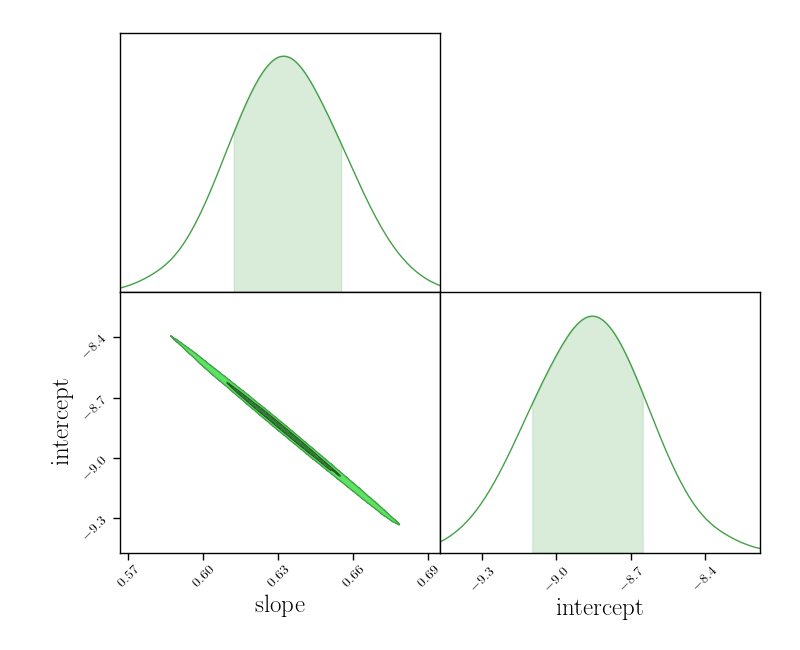
\includegraphics[width=0.5\textwidth]{figs/fit_fine_BC03_corner.png}
    \caption{Joint posterior distribution for the slope and intercept of the linear fit to the SN rate per galaxy per year as a function of stellar mass (Section \ref{sec:rates}; Fig. \ref{fig:rate_fitted}).}
    \label{fig:corner_slope_int}
\end{figure}
We model the relation with the linear relationship: 
\begin{equation}
    R_{\mathrm{G}} = \frac{\mathrm{d}R}{\mathrm{d}M_*} M_* + c \,,
\label{eq:rate_fit}
\end{equation}
where $dR/dM_*$ signifies the change of the rate of SNe as a function of the stellar mass, $c$ is a constant that sets the normalisation of the rate. We fit the model assuming a normal likelihood, such that the observed rate in each stellar mass bin is itself modelled as a Gaussian distribution described by the mean and standard deviation of the data in that bin. We adopt weakly informative normal priors on the slope and intercept: $p\left(\frac{\mathrm{d}R}{\mathrm{d}M_*}\right) \sim \mathcal{N}\left(0,5\right)$ and  $p\left(c\right) \sim \mathcal{N}\left(-12,5\right)$ respectively. We sample using 4 chains, each with 2000 warm up and 2000 sampling iterations. We report parameter estimates based on the mean and standard deviation of their posterior samples.

The joint posterior distribution for the slope and intercept are shown in Fig. \ref{fig:corner_slope_int}. The two parameters are highly degenerate, yet well constrained. This degeneracy manifests as the spread of potential linear fits as drawn in light blue on Fig. \ref{fig:rate_fitted}.

\section{Changes to the nominal SFH model}
\label{appendix:model_adjustments}
In Section \ref{sec:model} we describe our toy model of galaxy SFHs based on the work of \citet{Childress2014}. Here we 


%%%%%%%%%%%%%%%%%%%%%%%%%%%%%%%%%%%%%%%%%%%%%%%%%%


% Don't change these lines
\bsp	% typesetting comment
\label{lastpage}
\end{document}

% End of mnras_template.tex
